\documentclass[border=10pt]{standalone}

\usepackage{tikz}
\usepackage{tikzsymbols}
\usetikzlibrary{calc,patterns,shapes.geometric}

\def\centerarc[#1](#2)(#3:#4:#5){\draw[#1] ($(#2)+({#5*cos(#3)},{#5*sin(#3)})$) arc (#3:#4:#5);}

\begin{document}
	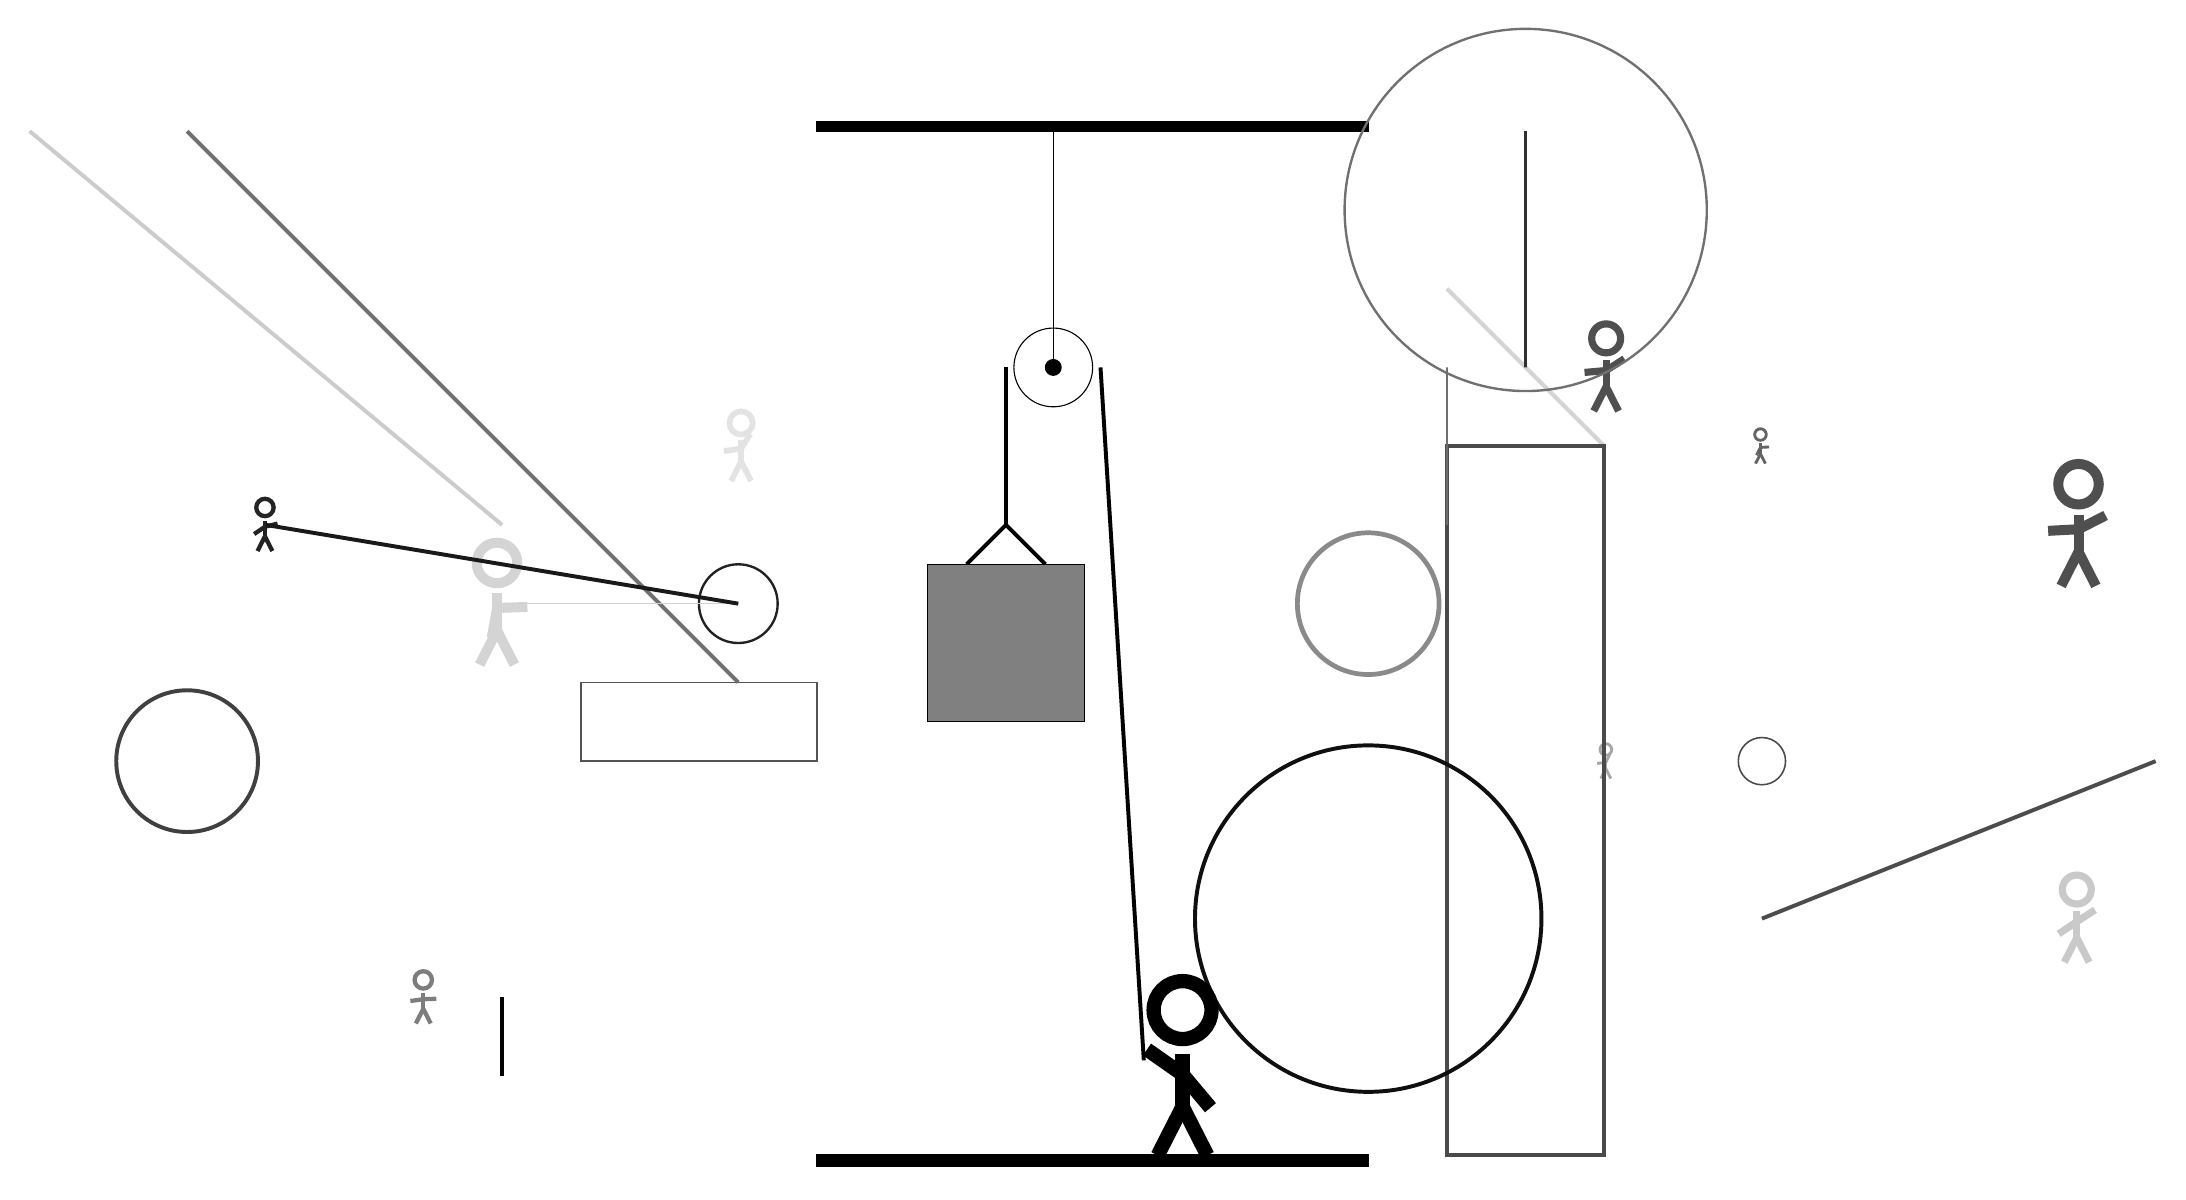
\begin{tikzpicture}
		%%%%% START %%%%%
		
		\draw[fill=black] (-2, 10) rectangle (5, 10.125);
		
		\node[line width=0.6mm, color=black!35] at (8, 2) {\Strichmaxerl[2][7][64]};
		
		\draw[line width=0.5mm, color=black!17](6, 8) -- (8, 6);
		\draw[line width=0.5mm, color=black!99](-6, -1) -- (-6, -2);
		\node[line width=0.7mm, color=black!11] at (-3, 6) {\Strichmaxerl[4][8][58]};
		\draw [line width=0.6mm, color=black!46](5, 4) circle (0.9);
		
		\node[line width=0.2mm, color=black!17] at (-6, 4) {\Strichmaxerl[7][80][2]};
		\node[line width=0.6mm, color=black!51] at (-7, -1) {\Strichmaxerl[3][8][2]};
		
		\draw[line width=0.2mm, color=black!67] (-2, 3) rectangle (-5, 2);
		\draw[line width=0.5mm, color=black!56](-3, 3) -- (-10, 10);
		\draw [line width=0.3mm, color=black!87](-3, 4) circle (0.5);
		
		\draw[line width=0.4mm, color=black!81] (7, 10) rectangle (7, 7);
		\node[line width=0.6mm, color=black!86] at (-9, 5) {\Strichmaxerl[3][34][14]};
		\node[line width=0.7mm, color=black!21] at (14, 0) {\Strichmaxerl[5][34][33]};
		
		\draw[line width=0.5mm, color=black!71] (6, -3) rectangle (8, 6);
		\node[line width=0.3mm, color=black!69] at (14, 5) {\Strichmaxerl[7][3][27]};
		\node[line width=0.6mm, color=black!69] at (8, 7) {\Strichmaxerl[5][5][33]};
		
		\draw [line width=0.3mm, color=black!56](7, 9) circle (2.3);
		\draw [line width=0.2mm, color=black!71](10, 2) circle (0.3);
		\draw[line width=0.2mm, color=black!18] (-3, 4) rectangle (-6, 4);
		
		\draw[line width=0.5mm, color=black!90](-3, 4) -- (-9, 5);
		\draw [line width=0.5mm, color=black!75](-10, 2) circle (0.9);
		
		\draw[line width=0.5mm, color=black!20](-6, 5) -- (-12, 10);
		\draw[line width=0.3mm, color=black!57] (6, 5) rectangle (6, 7);
		\draw [line width=0.5mm, color=black!94](5, 0) circle (2.2);
		\node[line width=0.6mm, color=black!61] at (10, 6) {\Strichmaxerl[2][63][3]};
		
		\draw[line width=0.5mm, color=black!70](10, 0) -- (15, 2);
		
		\draw (1, 7) circle (0.5);
		\draw[fill=black] (1, 7) circle (0.1);
		\draw (1, 10) -- (1, 7);
		
		\draw[line width=0.5mm] (-0.1, 4.5) -- (0.4, 5.0) -- (0.9, 4.5);
		\draw[fill=black!50] (-0.6, 4.5) rectangle (1.4, 2.5);
		
		\draw[line width=0.5mm] (0.4, 7) -- (0.4, 5.0);
		\centerarc[line width=0.5mm](1, 7)(0:180:0.6);
		\draw[line width=0.5mm](1.6, 7) -- (2.15, -1.8);
		
		\node at (2.6, -1.9) {\Strichmaxerl[10][-35][-50]};
		
		\draw[fill=black] (-2, -3) rectangle (5, -3.15);
		
		%%%%% END %%%%%
	\end{tikzpicture}
\end{document}